\documentclass[cjk,10pt]{beamer}
\usepackage{CJK}
\usepackage{latexsym, amsfonts, amssymb, amsmath,  amsthm}
\usepackage{amsopn, amstext, amscd,pifont}
\usepackage{amssymb,bm}
\usepackage{braket}
\usepackage{cases}
\usepackage{paralist}
\usepackage{eufrak}
\usepackage[all]{xy}
\usepackage[overload]{textcase}

\usepackage{chicago}
\bibliographystyle{chicago}


%\useoutertheme[height=1.5em]{sidebar}

\logo{
\includegraphics[scale=0.09]{nuslogo.pdf}}

\usetheme{Berkeley}
\useinnertheme{circles}
\usecolortheme{seahorse}
%\usecolortheme{dove}

\usefonttheme{professionalfonts}

\newtheorem{thm}[theorem]{Theorem}
\newtheorem{exa}[theorem]{Example}

\def\eqlaw{{\stackrel{\text{(law)}}{=}}}
\def\tmu{{\widetilde{\mu}}}
\def\tsigma{{\widetilde{\sigma}}}
\def\abs#1{{\left|#1\right|}}

\begin{document}
\setbeamertemplate{itemize subitem}[triangle]

\title{On quantiles of Brownian motion and \\
quantile options}
\author{Zhu Yong Ting}
\date{} \frame{\titlepage}

%\section{Outline}
%\begin{frame}
%\frametitle{Organization of this Thesis}
%
%%\begin{itemize}
%%\item Introduction  $\color{red}\surd$
%%\item Principles of option pricing 
%%\item Numerical methods
%%\item Quantile and quantile options $\color{red}\surd$
%%\item Conclusion and future work $\color{red}\surd$
%%\end{itemize}
%%\end{frame}


\section{Introduction} 
\begin{frame}{Definition of the quantile of a stochastic process}
\begin{itemize}
\item
For a stochastic process \{$X_t$\} on $(\Omega, \mathbb Q, \mathcal F)$, \\
\begin{equation}
M(\alpha,t)(\omega) = \inf\Set{x:\int_0^t 1_{\Set{X_s (\omega)\leq x}}ds > \alpha t},
\end{equation}
is the corresponding $\alpha$-quantile $(0 \leq \alpha \leq 1)$ process.
\item
Special cases:
\begin{itemize}
\item $\displaystyle\inf_{0\leq s \leq t}  X_s = \lim_{\alpha\to 0}M(\alpha,t)$
\item $\displaystyle\sup_{0\leq s \leq t} X_s = \lim_{\alpha\to 1} M(\alpha, t)$.
\end{itemize}
\item When $X_t = \sigma B_t + \mu t$ is a Brownian motion, many results are established. 
\end{itemize}
%Quantile options:
%Just replace the spot price by the quantiles.

%E.g. pay off function of 
%\begin{itemize}
%\item 
%$\alpha$-quantile European call option: $(S(\alpha,T)-K)^+$;
%\item 
%$\alpha$-quantile European call option: $(S(\alpha,\tau)-K)^+$.
% when execrice the option at time \tau
%\end{itemize}
\end{frame}

\begin{frame}{Motivation}
\begin{itemize}
\item
\cite{A-G-P-1995} examine the convergence behavior of the discretely sampled maximum of a Brownian motion. ($\alpha$=1)
\item
How are about the general $\alpha$-quantiles? ($\alpha \in (0,1)$)
\item
Part I: Discretization error in simulation of the quantile of a Brownian motion.
\end{itemize}
%Key property:
%\[
%(M(\alpha,T),X_T) 
%{\stackrel{\text{(law)}}{=}}
% (\max_{t\leq \alpha T}X_t+\min_{t\leq (1-\alpha)T}X'_t, X_{\alpha T}+X'_{(1-\alpha)T}),
%\]
%where $X'_t$ is an independent copy of $X_t$. 
\end{frame}

\begin{frame}{Motivation}
\begin{itemize}
\item
Lognormal stock price model: 

Stock price $S_t$ satisfies 
\[
S_t=S_0\exp((r-\sigma^2 /2)t + \sigma B_t)
\]

with $r$ and $\sigma $ constant, which represent the risk free interest rate and the volatility respectively. 

\item
Quantile option: quantile of stock price ($\alpha \in (0,1)$)

\item
Part II: Pricing of American-style $\alpha$-quantile option
\end{itemize}
\end{frame}



%
%\begin{frame}{Discretization}
%Discretize the continuous stochastic process( Brownian motion)
%\[
%X_{i,h} = X_{ih}
%\]
%is a discrete stochastic process(Gaussian random walk),
% where $h$ is the step length.
%
%
%$M_h(\alpha,T)$: the $k=\alpha T/h$-th order statistic of the set 
%$\Set{X_{i,h}|n=0,1,\cdots, T/h}$.
%
%Similar property ($h=T/N$,$k=\alpha N$)
%\[
%(M_h(1,T),X_{N,h}) 
%{\stackrel{\text{(law)}}{=}}
% (\max_{i\leq k}X_{i,h}+\min_{i\leq N-k}X'_{i,h}, X_{k,h}+X'_{N-k,h}),
%\]
%\end{frame}


\section{Discretization error}
%\begin{frame}{Euler scheme and random walk}
%For a process $Y=\{Y(t)\}_{t\geq 0}$ satisfying the SDE 
%\begin{equation}
%dY(t)= b(Y(t))dt + \sigma (Y(t))dB_t,
%\end{equation}
%with initial condition $Y(0)=y$, the approximation $Y_h = \{Y_h (t)\}_{t\geq 0}$ to $Y$ in the Euler scheme is defined as
%\begin{equation}
%Y_h ((k+1)h) = Y_h (kh) + b(Y_h(kh))h + \sigma(Y_h(kh))(B_{(k+1)h}-B_{kh}),
%\end{equation}
%on the grid $h\mathbb N$, $Y_h (t) = Y_h (\lfloor t/h \rfloor h)$ off the grid and $Y_h (0) = y$.

%Obviously, the accuracy of this approximation is closely related to the length of the discretized time increment $h$. Then the questions arise: how fine should the discretized time increment be in order to get a satisfactory approximation and whether we can quantify the accuracy of this type of simulation. To address this question, the discretization error is introduced. 

%\end{frame}
\subsection{The quantile of a Brownian motion}
\begin{frame}{The distribution function}
For a Brownian motion without drift ($\mu=0$, $X_t=\sigma B_t$), \cite{Yor1995} provides the distribution function:
\vspace{1em}
%For the $\alpha$-quantile $M(\alpha,t)$ of $\{X_t\}$ on time interval $[0,t]$
{\small
\begin{equation}
P(M(\alpha,t)\in dx)= \begin{cases}
\displaystyle 2\sqrt\frac{2}{\sigma^2\pi t}\exp\left(\frac{-x^2} {2\sigma^2 t}\right)\left(1-\Phi\left(\frac{|x|} {\sigma^2 t\theta}\right)\right)dx  &  \text{if } x \leq 0 ,\\
\displaystyle 2\sqrt\frac{2}{\sigma^2\pi t}\exp\left(\frac{-x^2} {2\sigma^2 t}\right)\left(1-\Phi\left(\frac{\theta x}{\sigma^2 t}\right)\right)dx  & \text{if } x \geq 0,
\end{cases}
\end{equation}
}
where $\theta = ((1 - \alpha)/\alpha)^{1/2}$ and $\Phi(x)=\int^{x}_{-\infty}(2\pi)^{(-1/2)}\exp(-y^2 /2)dy$ is the cumulative distribution function of a standard normal random variable.
\end{frame}

\begin{frame}{The density function}
For general Brownian motion, \cite{Dassios1995} proved that
\begin{equation}\label{eq:Dassios}
M(\alpha, t) \eqlaw \sup_{s \leq \alpha t} X_s + \inf_{s\leq (1-\alpha)t} X'_s ,
\end{equation}
where $X'$ is a independent copy of $X$.
\end{frame}


\begin{frame}{The density function}
The density function of $\alpha$-quantile $M(\alpha,t)$ of a Brownian motion is 
\begin{equation}\label{eq:fulldensity}
g(x; \alpha , t) = \int^{\infty}_{-\infty} g_1 (x-y; \alpha t) g_2 (y; (1-\alpha) t)dy ,
\end{equation}
where
\begin{equation}
g_1 (x;t) = \begin{cases}
\displaystyle\frac{1}{\sigma}\left({\frac{2}{\pi t}}\right)^{1/2}\exp\left\{-\frac{(x-\mu t)^2}{2\sigma ^2 t}\right\} \\
\displaystyle\quad - \frac{2\mu}{\sigma ^2} \exp\left(\frac{2\mu x}{\sigma ^2}\right)\left[1- \Phi \left(\frac{x+\mu t}{\sigma \sqrt{t}}\right)\right], & x > 0 ,\\
0 , & x  \leq 0 ,
\end{cases}
\end{equation}

\begin{equation}
g_2 (x;t) = \begin{cases}
0, & x \geq 0 \\
\displaystyle\frac{1}{\sigma}\left({\frac{2}{\pi t}}\right)^{1/2}\exp\left\{-\frac{(x-\mu t)^2}{2\sigma ^2 t}\right\} \\
\displaystyle\quad + \frac{2\mu}{\sigma ^2} \exp\left(\frac{2\mu x}{\sigma ^2}\right) \Phi \left(\frac{x+\mu t}{\sigma \sqrt{t}}\right) , & x < 0.
\end{cases}
\end{equation}
\end{frame}


\begin{frame}{Euler approximation of quantiles}
\begin{itemize}
\item
Euler scheme:
\begin{itemize}
\item
Divide the time interval $[0,T]$ into $N$ equal small time intervals with length $h$. 
\item
The Euler approximation for the $\alpha$-quantile $M(\alpha, T)$ of the Brownian motion $\{X_t\}_{t\leq T}$ is the $k$-th order statistic of the set $\{X_{nh},n=0,1,\cdots,N\}$ with $k= \lceil \alpha  N\rceil$. 
\end{itemize}
\item
Denote $M(k,N)$ as the Euler approximation of $M(\alpha, T)$ with $h=T/N$. 
\item
How fine should the discretized time increment be in order to get a satisfactory approximation?
\item
How to quantify the accuracy of this type of approximation?
\end{itemize}
\end{frame}

\begin{frame}{Discretization error and order of convergence}
\begin{itemize}
\item
The discretization error for the Euler approximation of the $\alpha$-quantile of a Brownian motion at time $T$ is 
\begin{equation}
\varepsilon_N =M(\alpha, T)-M(k,N).
\end{equation}
\item
The quality of a path-wise approximation at time $T$ can be measured by 
\begin{equation}\label{strong-g}
\mathbb E|\varepsilon_N| =E|M(\alpha, T)-M(k,N)|.
\end{equation}
\item
If (\ref{strong-g}) is $O(1/N^\gamma)$ as $N \uparrow \infty$, this approximation is said to {\it converge strongly} with order $\gamma > 0 $ at time $T$.
%Using an identity from \cite{Wendel1960} about random walks with independent and identically distributed increments, it can be established that 
%\begin{equation}\label{eq:dpathdec}
%M(k,N)\stackrel{\rm(law)}{=}\max_{i\le k}X_{ih} + \min_{i\le N-k}X'_{ih},
%\end{equation}
%where $X'$ is an independent copy of $X$. 
\end{itemize}
\end{frame}



\begin{frame}{Results for maximum}
\begin{itemize}
\item
\cite{A-G-P-1995} find that \[E[M(1,T)-M(N,N)] = O(1/N^{1/2})\] as $N\to\infty$. 
\item
{\color{red} Question:} What about the general $\alpha$-quantiles ($\alpha \in (0,1)$)? 
\end{itemize}
\end{frame}

\subsection{Numerical study}
\begin{frame}{A numerical study about the strong order of convergence}
\begin{itemize}
\item
The strong order is related to 
\begin{equation}
\mathbb E|\varepsilon_N| =E|M(\alpha, T)-M(k,N)|.
\end{equation}
\item
Sampled $M(\alpha,T)$ and $M(k,N)$ should share the same path. 
\item
We use a much finer Euler approximation as an approximation of the continuous $\alpha$-quantile $M(\alpha, T)$. 
\end{itemize}
\end{frame}


\begin{frame}{The algorithm}
\small
\begin{itemize}
\item 
The parameter setting is : 
\begin{equation}
 N = 2^b , 2^{b+1} , ... 2^{d}; 
\alpha_j =  \frac{1}{2} + \frac{j}{2^b} , j = 0, 1 , 2..., 2^{b-1}.
\end{equation}
\item
The algorithm: 
\begin{itemize}
\item Generate $2^{d}$ normal random sample $\Set{x_i}$ 
  with mean $\tmu=\mu/2^d$,
  and standard deviation $\tsigma = \sigma \sqrt {{T}/{2^d}}$,
  add them up according to time and record them as
  $X_m = \sum_{1\leq i \leq m} x_i$ starting with $X_0$.
\item Calculate the $\alpha_j$ quantiles 
  $M_{j,s}\triangleq M_{\alpha_j 2^s,2^s}$ for sequence 
  \[
  \Set{X_m|m=i 2^{d-s}, 1\leq i\leq 2^{s}},\quad \text{where }b\leq s \leq d.\] 
\item Use $M_{j,d}$ as the continuous quantiles $M(\alpha_j,T)$.
\item Repeat the above for $L$ times,
  get replicates $\Set{M_{j,s}^{(l)},{1\leq l\leq L}}$.
\item Approximate the expectation of the absolute discretization error for $s < d$ using:
\begin{align}
Err^{abs}_{j,s} &= \frac{1}{L}\sum_{1\leq l \leq L} \abs{M_{j,d}^{(l)}- M_{j,s}^{(l)}}.
\end{align}
\end{itemize}
\end{itemize}
\end{frame}

%\begin{frame}
%When $T/h \in \mathbb{N}$, we have 
%\[
%\mathbb{E}\left( M(\alpha, T) - M_h(\alpha,T)\right) 
%= 
%\begin{cases}
%O(h^{1/2}) & \alpha=0,1\\
%0 & \alpha=0.5\\
%O(h) & \text{otherwize}
%\end{cases} 
%\]
%
%Conclusion: The convergence patten of genuine $\alpha$-quantiles are different
%with the extrema case. 
%\end{frame}

\begin{frame}{Numerical results for $\mu=0$}
\begin{figure}
   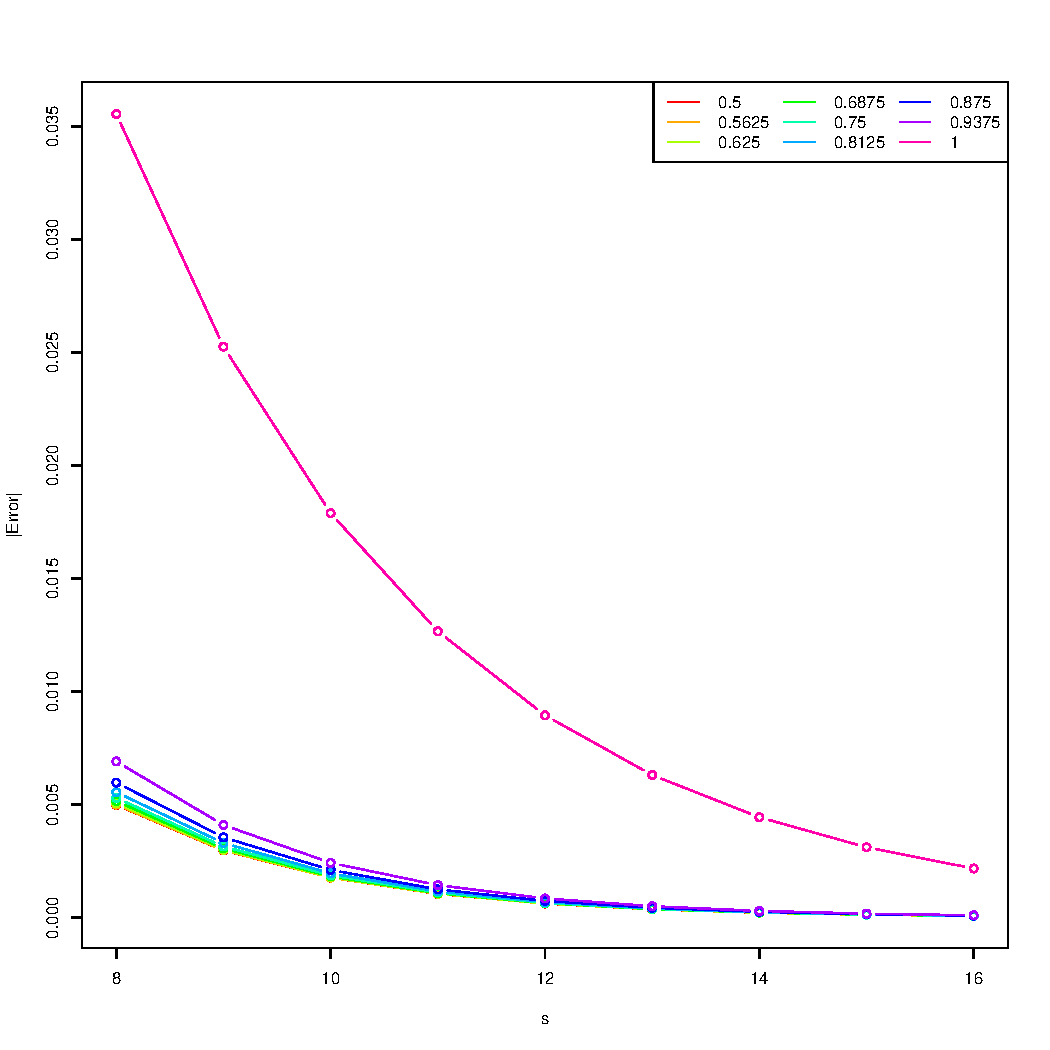
\includegraphics[scale=0.3]{nout_0a.pdf}
   \caption{Expectation of the absolute discretization error for selected $\alpha$-quantiles ($\alpha = 0.5, 0.5625, \cdots, 1$) using the Euler scheme with $N = 2^s$ ($4\le s \le 16$), $\mu=0$, $\sigma=1$, $T=1$, $X_0=0$ and $L=500000$. }
\label{f:ab}
\end{figure}
\end{frame}

\begin{frame}{The logarithm treatment}
\begin{itemize}
\item
Suppose the expectation of the absolute discretization error is $O(1/N^\gamma)$, then we get
\begin{equation}\label{error-N-sim}
E|\varepsilon_N| \approx C/N^\gamma,
\end{equation}
where $C$ is some positive constant. 
\item
Considering in our simulation $N$ is $N = 2^s$, take logarithm to both sides of (\ref{error-N-sim}) we get
\begin{equation}
\log_2 E|\varepsilon_{2^s}| \approx \log_2 C -\gamma s
\end{equation}
\end{itemize}
\end{frame}


\begin{frame}{Numerical results for $\mu=0$}
 \begin{figure}
   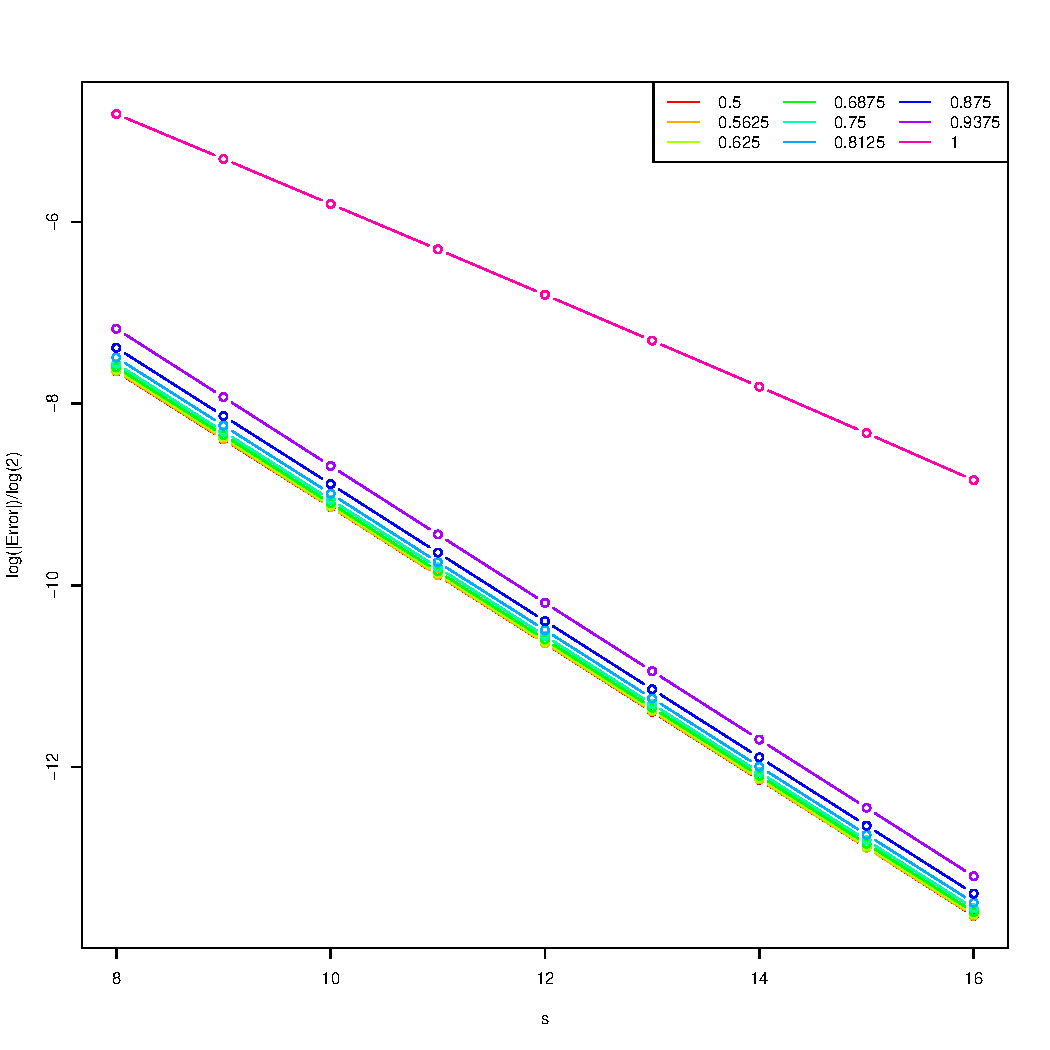
\includegraphics[scale=0.3]{nout_0alog.pdf}
   \caption{Logarithm of the absolute discretization error for selected $\alpha$-quantiles ($\alpha = 0.5, 0.5625, \cdots, 1$) using the Euler scheme with $N = 2^s$ ($4\le s \le 16$), $\mu=0$, $\sigma=1$, $T=1$, $X_0=0$, $L=500000$.} 
   \label{f:lab}
\end{figure}
\end{frame}

\begin{frame}{Numerical results for $\mu=0$}
 \begin{figure}[p]
   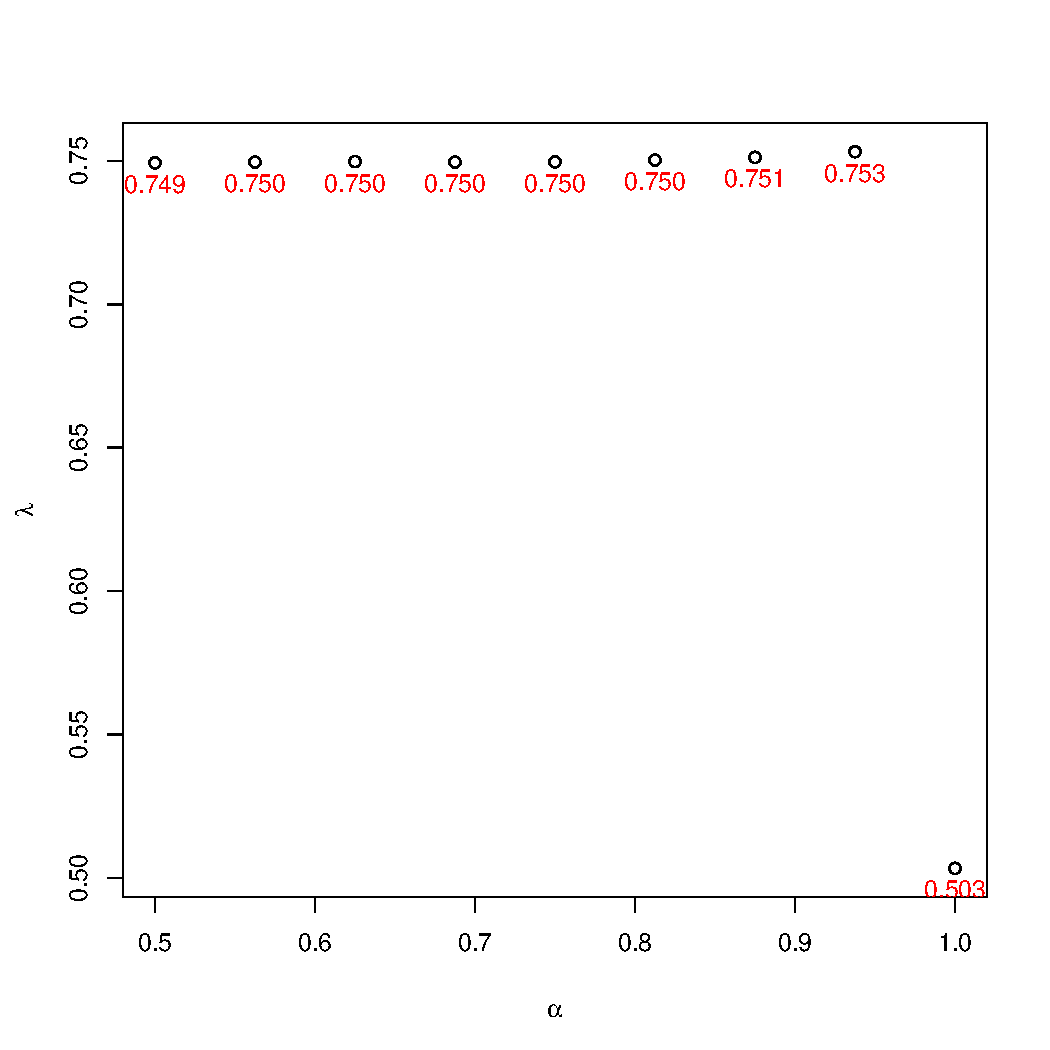
\includegraphics[scale=0.3]{nout_0arato.pdf} % requires the graphicx packagem 
   \caption{The strong order of convergence for selected $\alpha$-quantiles ($\alpha $ $=$ $ 0.5,$ $0.5625,$ $\cdots, 1$) using the Euler scheme with $N = 2^s$ ($4\le s \le 16$), $\mu=0$, $\sigma=1$, $T=1$, $X_0=0$, $L=500000$.}
   \label{f:ratio}
\end{figure}
\end{frame}

%\begin{frame}{Numerical results for $\mu=3$}
%\begin{figure}[p]
%   %\centering
%   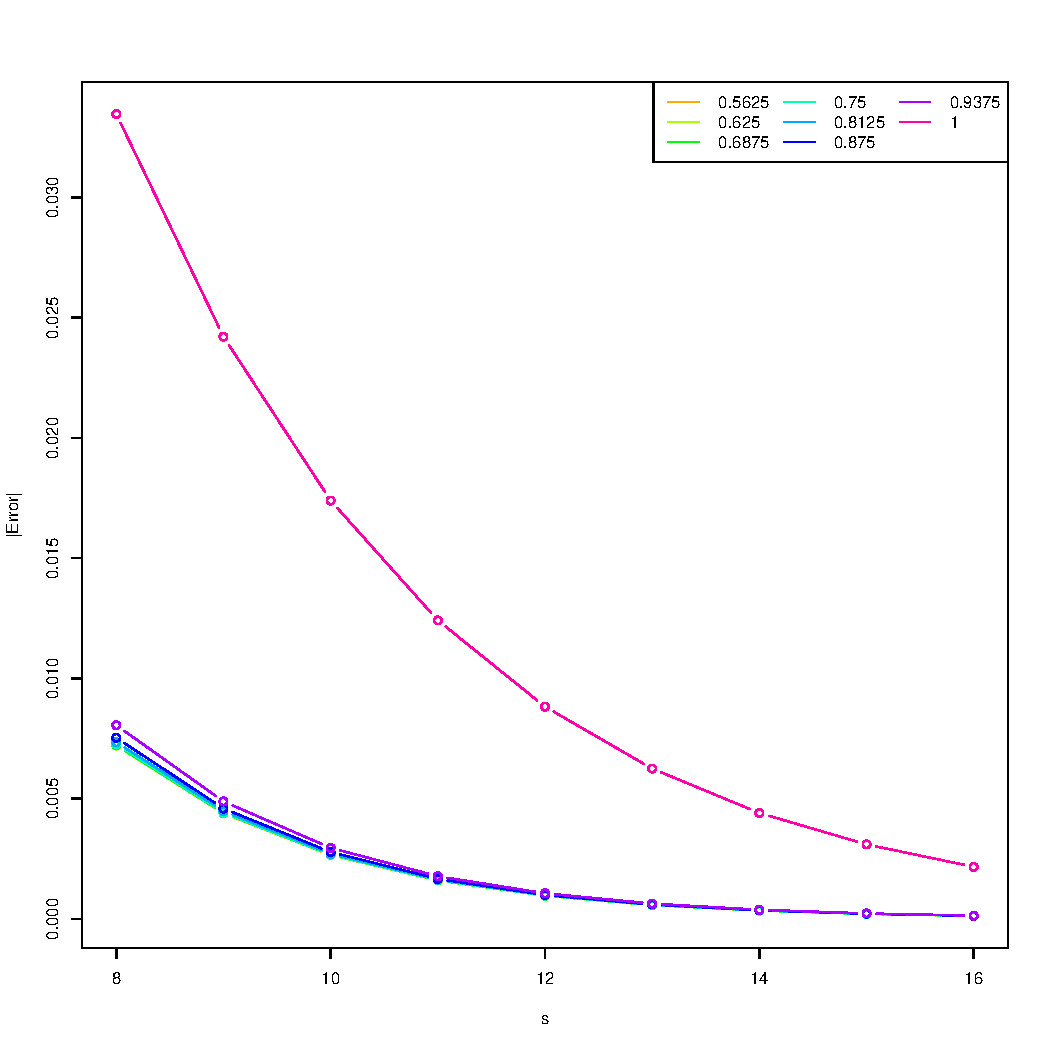
\includegraphics[scale=0.3]{nout_4_25_3a.pdf}
%   \caption{Expectation of the absolute discretization error for selected $\alpha$-quantiles ($\alpha = 0.5, 0.5625, \cdots, 1$) using the Euler scheme with $N = 2^s$ ($4\le s \le 16$), $\mu=3$, $\sigma=1$, $T=1$, $X_0=0$, $L=500000$. }
%\label{f:ab3}
%\end{figure}
%\end{frame}
%
%\begin{frame}{Numerical results for $\mu=3$} 
%\begin{figure}[p]
%    %\centering
%   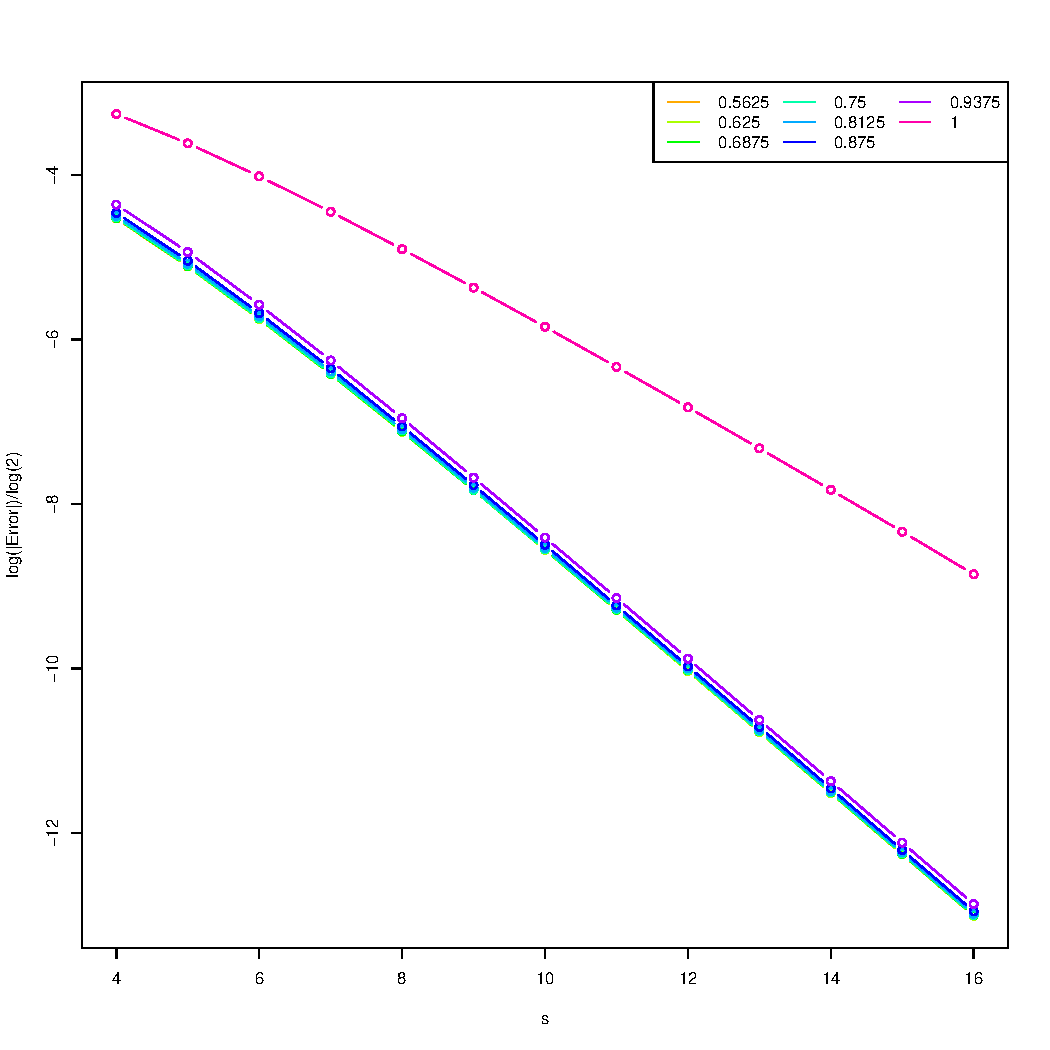
\includegraphics[scale=0.3]{nout_4_25_3alog.pdf}
%   \caption{Logarithm of the absolute discretization error for selected $\alpha$-quantiles ($\alpha = 0.5, 0.5625, \cdots, 1$) using the Euler scheme with $N = 2^s$ ($4\le s \le 16$), $\mu=3$, $\sigma=1$, $T=1$, $X_0=0$, $L=500000$.} 
%   \label{f:lab3}
%\end{figure}
%\end{frame}
% 
%\begin{frame}{Numerical results for $\mu=3$} 
%\begin{figure}[p]
%   %\centering
%   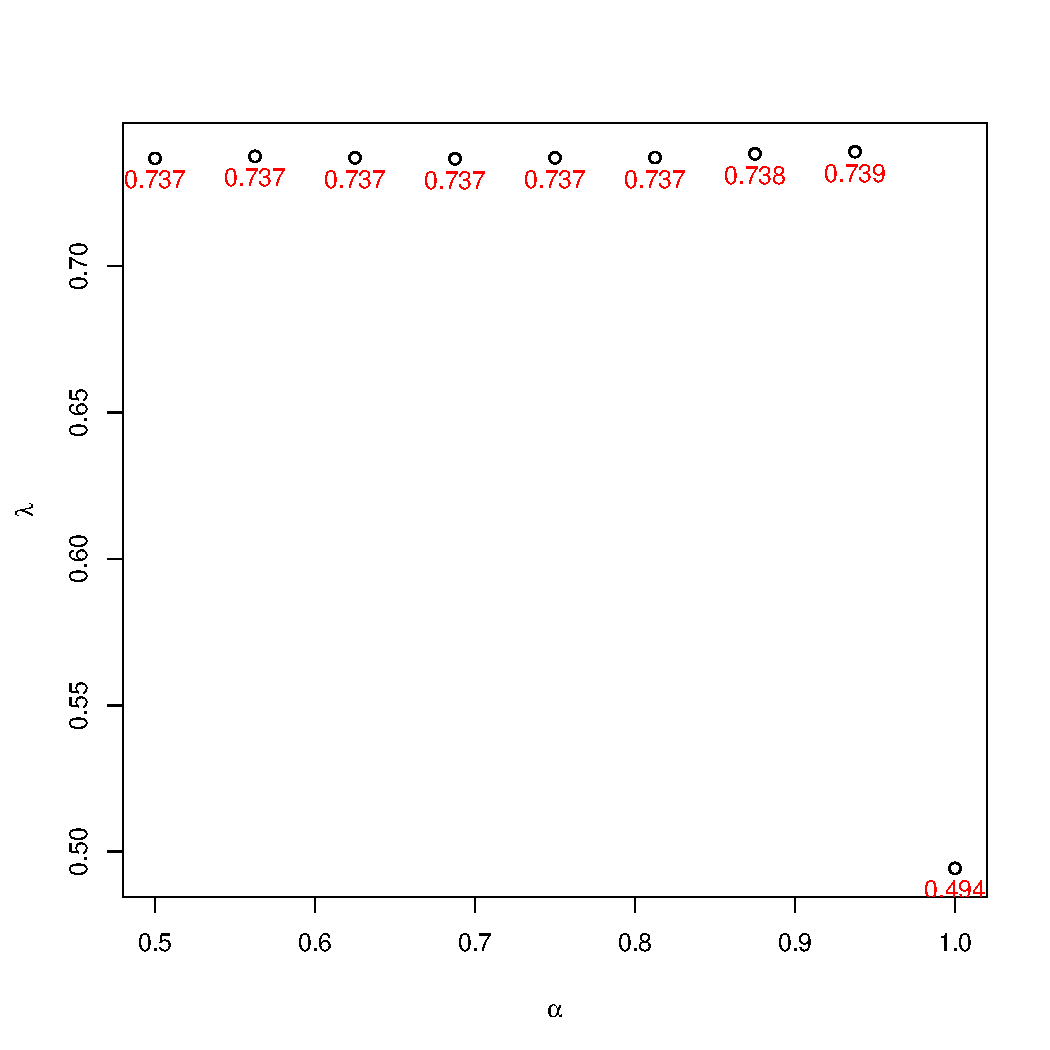
\includegraphics[scale=0.3]{nout_4_25_3arato.pdf} % requires the graphicx packagem 
%   \caption{The strong order of convergence for selected $\alpha$-quantiles ($\alpha = 0.5, 0.5625, \cdots, 1$) using the Euler scheme with $N = 2^s$ ($4\le s \le 16$), $\mu=3$, $\sigma=1$, $T=1$, $X_0=0$, $L=500000$.}
%   \label{f:ratio3}
%\end{figure}
%\end{frame}

\begin{frame}{Conclusion from numerical study}
\begin{itemize}
\item
The strong order of convergence for the maximum is around $1/2$.
\item
Moreover, for other quantiles, the strong order of convergence is far away from $1/2$, all of them are around to $0.75$.
\item
These simulations reflected the huge difference of strong order of convergence for genuine quantiles and the maximum of a Brownian motion.
\end{itemize}
\end{frame}

\subsection{Theoretical study}
\begin{frame}{An analysis about the expected discretization error}\small
\begin{itemize}
\item 
\cite{Dassios1995} 
\[
M(\alpha, T) \eqlaw \sup_{s \leq \alpha T} X_s + \inf_{s\leq (1-\alpha)T} X'_s.
\]
\item
\cite{Wendel1960}
\[
M(k,N)\stackrel{\rm(law)}{=}\sup_{i\le k}X_{ih} + \inf_{i\le N-k}X'_{ih}.
\]

\item
\cite{Janssen2008}
\begin{itemize}
\item$\displaystyle
E[M(1,T)-M(N,N)]
= -\frac{\zeta(1/2)}{\sqrt{2\pi}}\sigma\sqrt{T/N} 
 -\frac{2g(\mu\sqrt{T}/\sigma)-\mu\sqrt{T}/ \sigma}{4N}\sigma\sqrt{T} 
 +O(1/N^{3/2}),$
where 
$
\zeta(1/2) \approx -3.92264613,
$
and 
$
g(x)=x \Phi(x) + \frac{1}{\sqrt{2\pi}} e^{-{x^2 /2 }}.
$
\item
The expected discretization error of the maximum of a Brownian motion is symmetric w.r.t drift $\mu$.
\end{itemize}
\end{itemize}
\end{frame}

\begin{frame}\small
We find 
\begin{itemize}
\item
\begin{equation}
\mathbb {E}({M(1-\alpha,T) - M(N-k,N)})
=-\mathbb{E}({M(\alpha,T) -  M(k,N)}).
\end{equation}
\item
The discretization error of $\alpha$-quantile of Brownian motion with drift $\mu$ is the same as that of Brownian motion with drift $-\mu$.

\item
for $\alpha=0.5$, 
\begin{equation}
\mathbb{E} [{M(0.5,T) - M(N/2,N)}]=0.
\end{equation}

\item
for $0<\alpha<1$,
\begin{equation}
\begin{split}
&\mathbb{E} [{M(\alpha,T) -  M(k,N)}]\\
=&\frac{\sigma\sqrt{T}}{4N}\left(\frac{(\mu_1 - 2g(\mu_1))}{\sqrt\alpha} - \frac{(\mu_2 - 2g(\mu_2))}{\sqrt{(1-\alpha)}}\right) \\
& + O(1/N^{{3}/{2}}),
\end{split}
\end{equation}
where $k = \alpha N$, $\mu_1 =\mu\sqrt{\alpha T}/\sigma$, and $\mu_2 =-\mu\sqrt{(1-\alpha)T}/\sigma$.

\end{itemize}
\end{frame}

\begin{frame}{The coefficient}
\begin{figure}[p]
   %\centering
   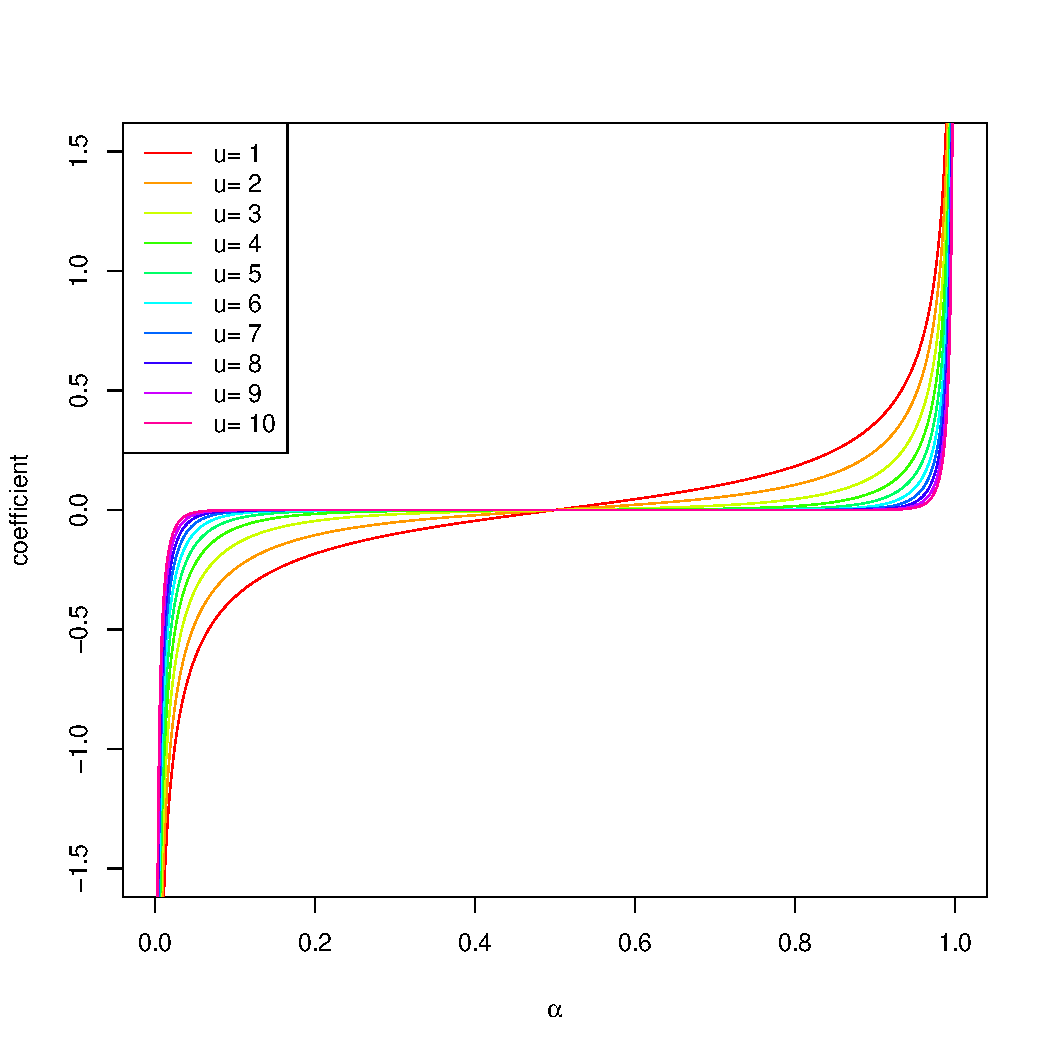
\includegraphics[scale=0.3]{mu.pdf} % requires the graphicx packagem 
   \caption{Coefficient of the leading term}
   \label{plot-mu}
\end{figure}
\end{frame}


\begin{frame}{Numerical results for $\mu=0$}
\begin{figure}
   \centering
   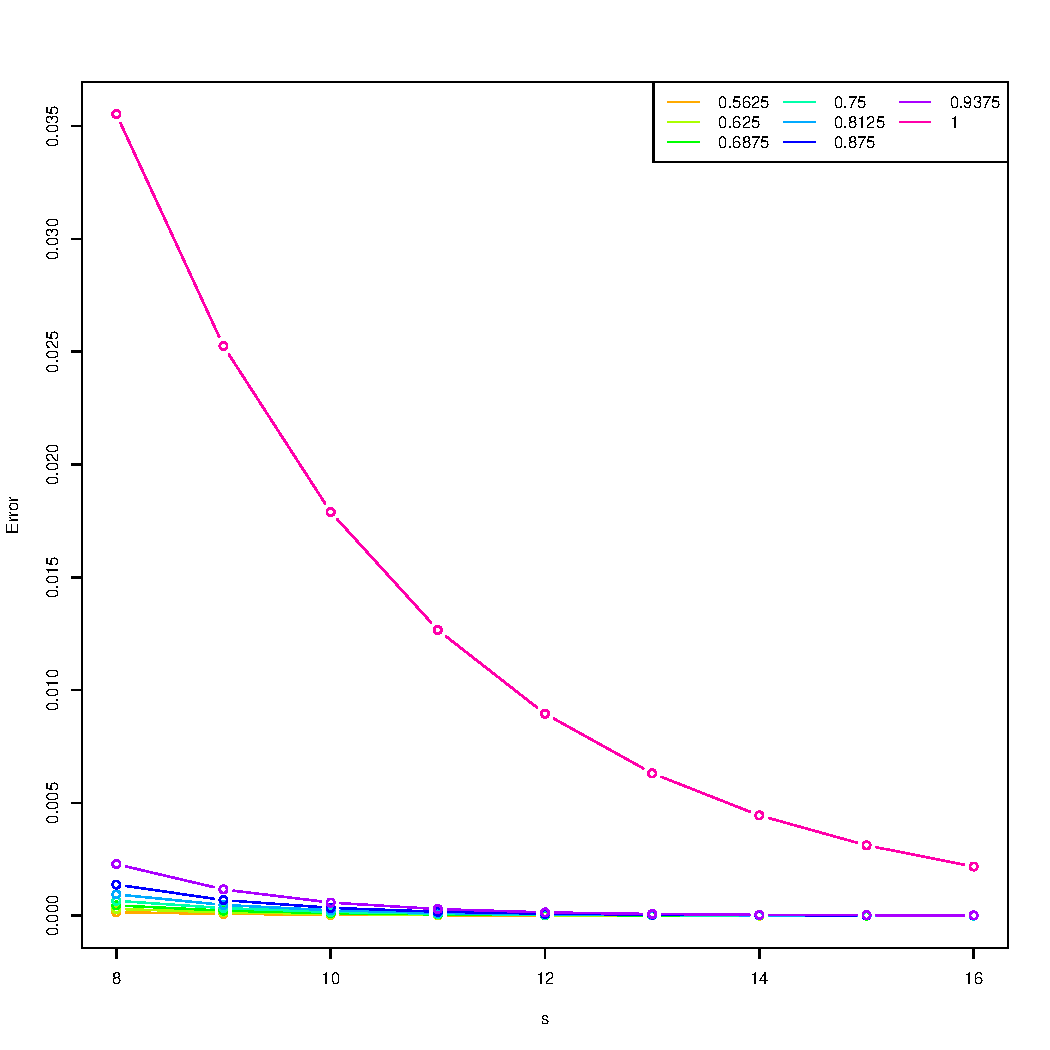
\includegraphics[scale=0.3]{nout_0.pdf} % requires the graphicx package
   \caption{Expectation of the discretization error for selected $\alpha$-quantile ($\alpha = 0.5625, 0.625, \cdots, 1$) using the Euler scheme with $N = 2^s$ ($4\le s \le 16$), $\mu=0$, $\sigma=1$, $T=1$, $X_0=0$, $L=500000$ }
   \label{f:err}
\end{figure}
\end{frame}

\begin{frame}{Numerical results for $\mu=0$}
\begin{figure}
   \centering
   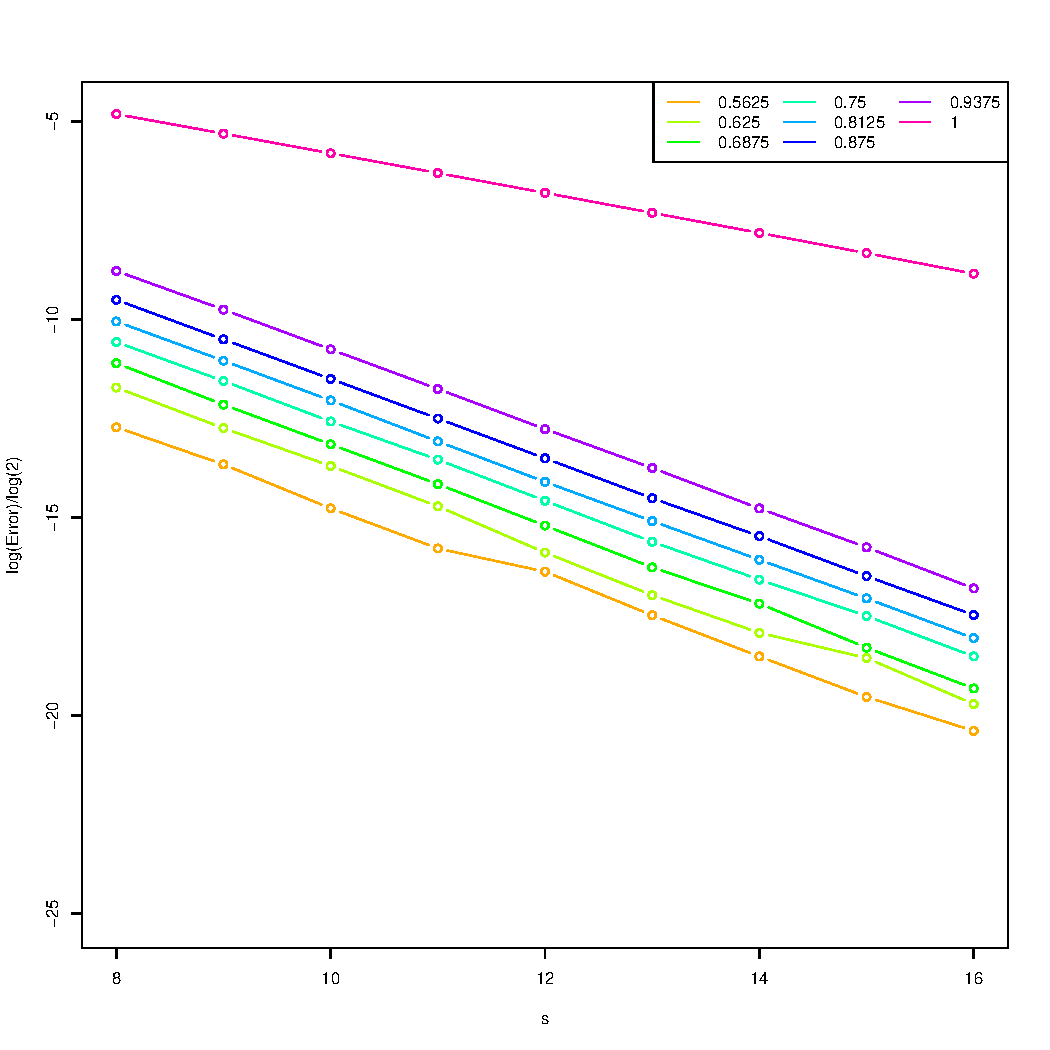
\includegraphics[scale=0.3]{nout_0log.pdf} % requires the graphicx package
   \caption{Logarithm of the discretization error for selected $\alpha$-quantile ($\alpha =$ $0.5625,$ $0.625,$ 
   $\cdots, 1$) using the Euler scheme with $N = 2^s$ ($4\le s \le 16$), $\mu=0$, $\sigma=1$, $T=1$, $X_0=0$, $L=500000$}
   \label{f:lerr}
\end{figure}
\end{frame}

\begin{frame}{Numerical results for $\mu=0$}
\begin{figure}
   \centering
   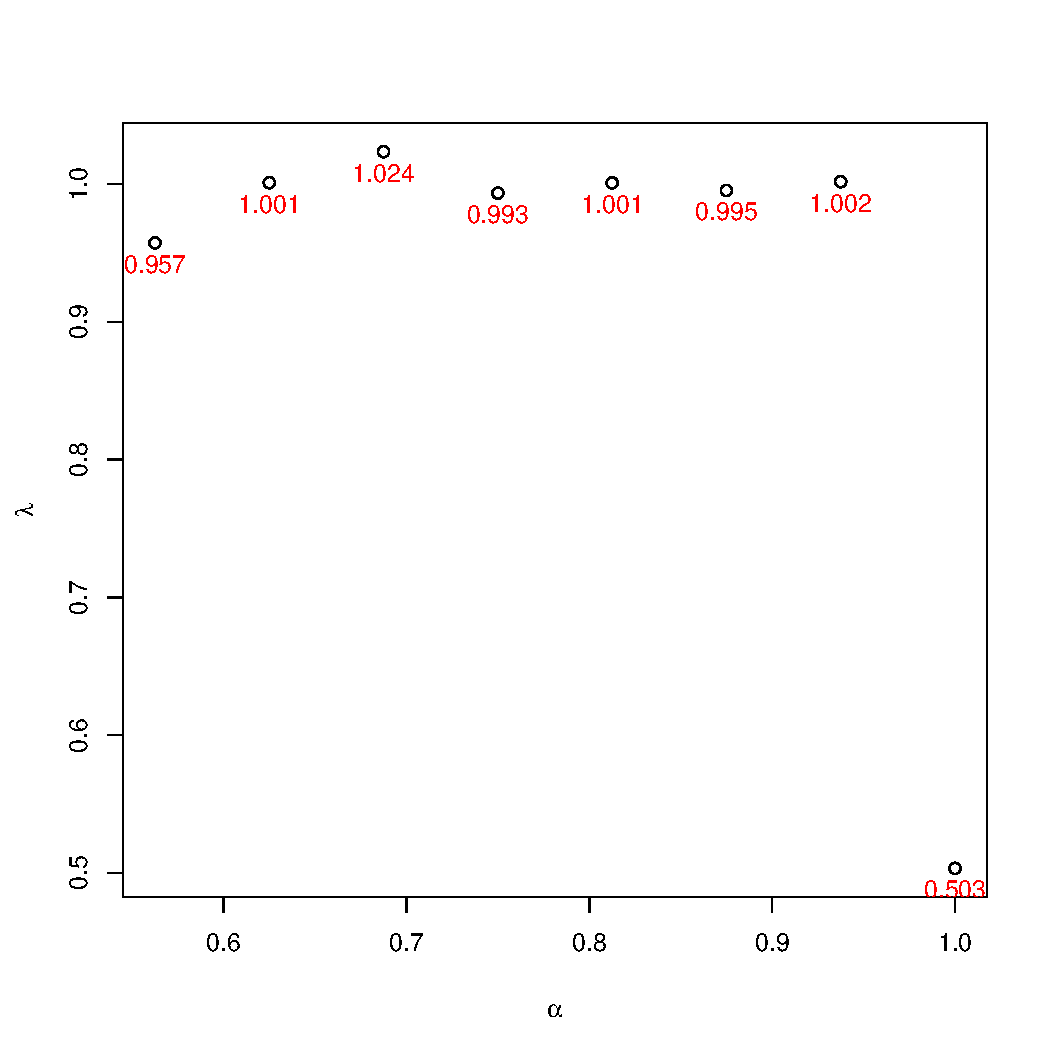
\includegraphics[scale=0.3]{nout_0rato.pdf} % requires the graphicx package
   \caption{The order of convergence for selected $\alpha$-quantile ($\alpha = 0.5625, 0.625,  \cdots, 1$) using the Euler scheme with $N = 2^s$ ($4\le s \le 16$), $\mu=0$, $\sigma=1$, $T=1$, $X_0=0$, $L=500000$}
   \label{f:rate}
\end{figure}
\end{frame}

%\begin{frame}{Numerical results for $\mu=3$}
%\begin{figure}[p]
%   \centering
%   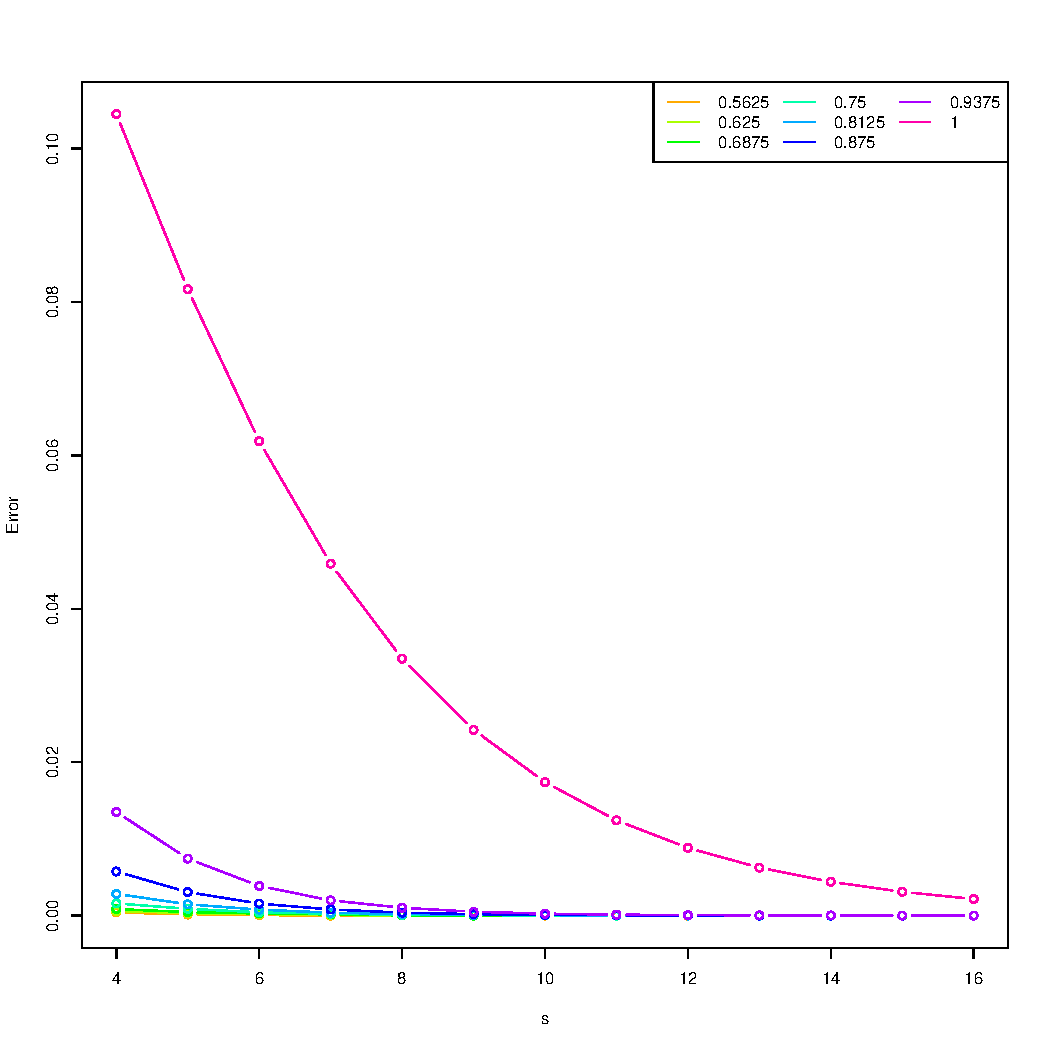
\includegraphics[scale=0.3]{nout_4_25_3.pdf} % requires the graphicx package
%   \caption{Expectation of the discretization error for selected $\alpha$-quantile ($\alpha = 0.5625, 0.625,  \cdots, 1$) using the Euler scheme with $N = 2^s$ ($4\le s \le 16$), $\mu=3$, $\sigma=1$, $T=1$, $X_0=0$, $L=500000$ }
%   \label{f:err3}
%\end{figure}
%\end{frame}
%
%\begin{frame}{Numerical results for $\mu=3$}
%\begin{figure}[p]
%   \centering
%   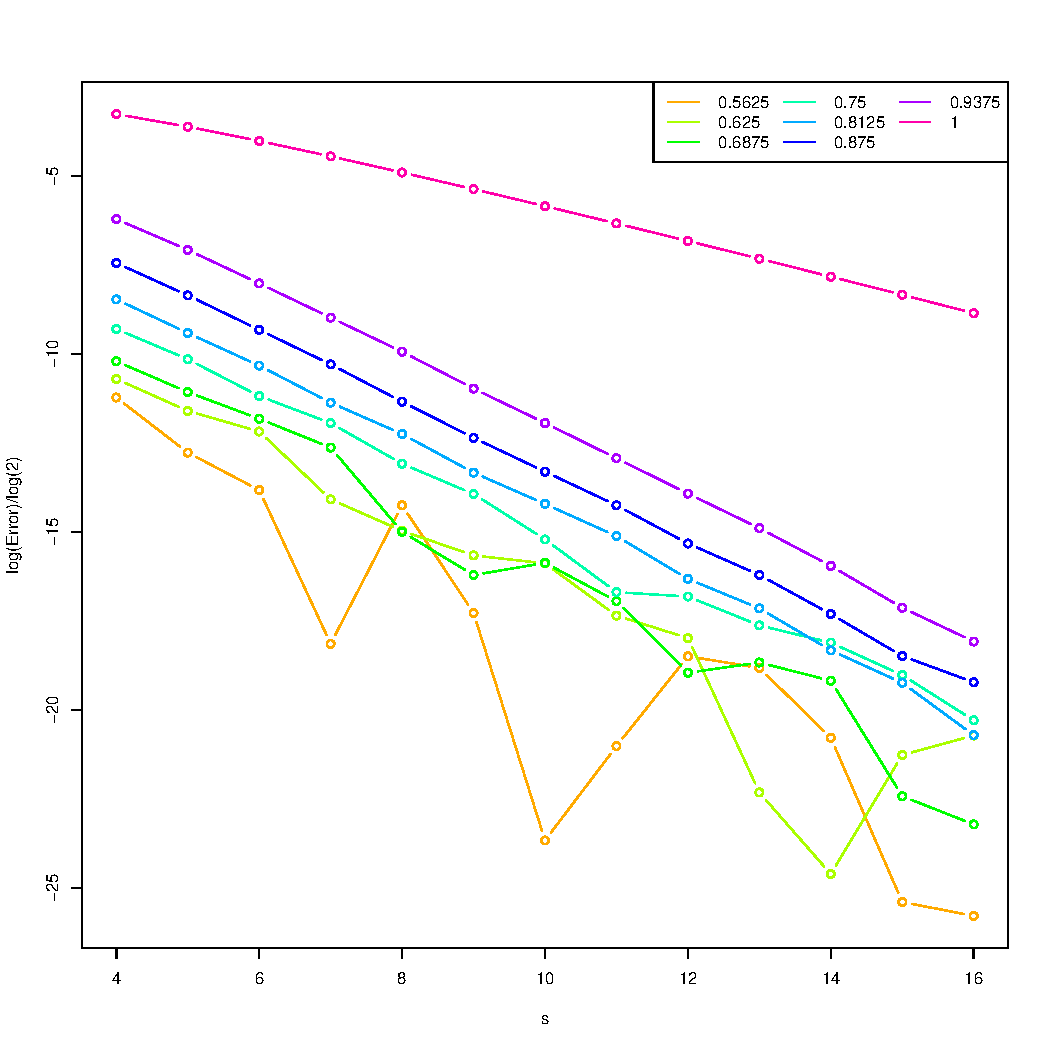
\includegraphics[scale=0.3]{nout_4_25_3log.pdf} % requires the graphicx package
%   \caption{Logarithm of the discretization error for selected $\alpha$-quantile ($\alpha =$ $0.5625,$ $0.625,$  $\cdots, 1$) using the Euler scheme with $N = 2^s$ ($4\le s \le 16$), $\mu=3$, $\sigma=1$, $T=1$, $X_0=0$, $L=500000$}
%   \label{f:lerr3}
%\end{figure}
%\end{frame}
%
%\begin{frame}{Numerical results for $\mu=3$}
%\begin{figure}[p]
%   \centering
%   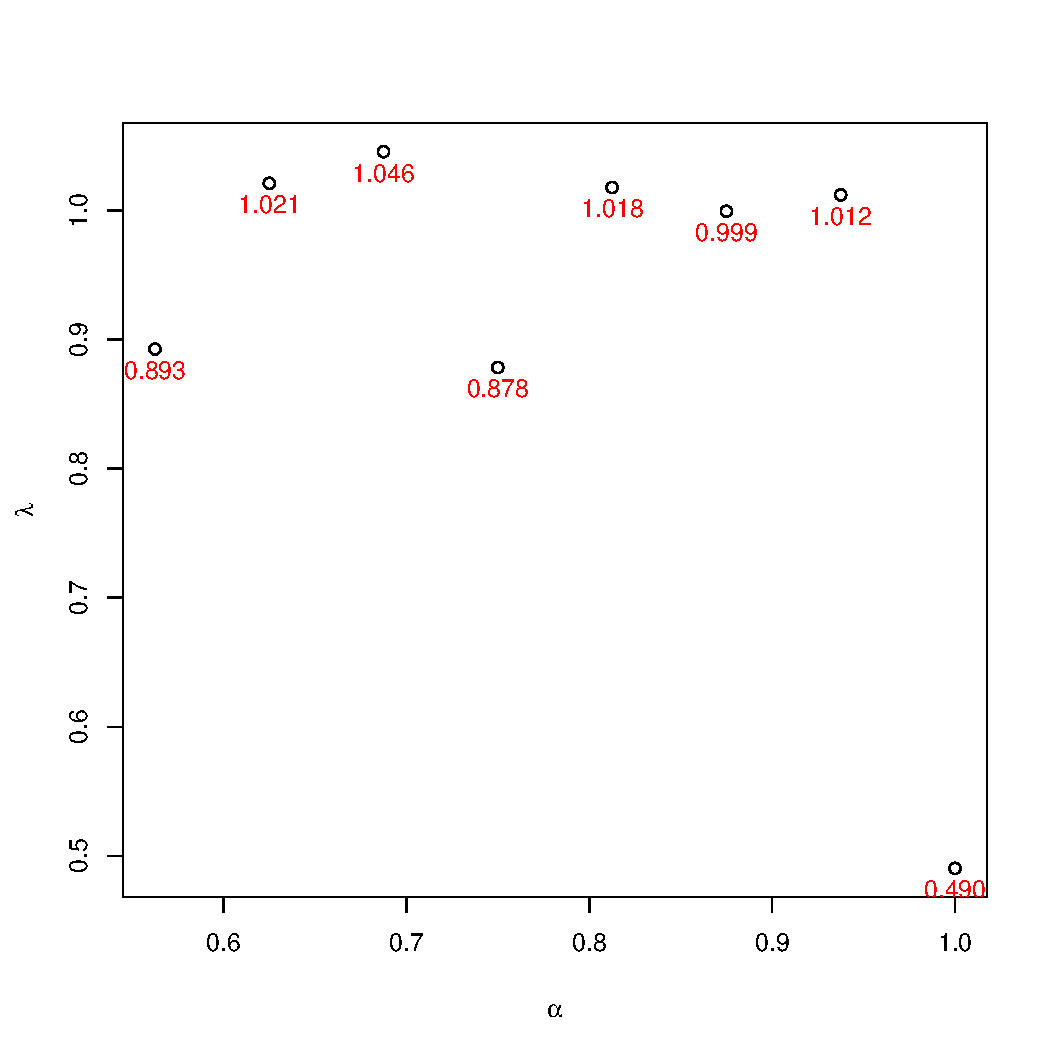
\includegraphics[scale=0.3]{nout_4_25_3rato.pdf} % requires the graphicx package
%   \caption{The order of convergence for selected $\alpha$-quantile ($\alpha = 0.5625, \cdots, 1$) using the Euler scheme with $N = 2^s$ ($4\le s \le 16$), $\mu=3$, $\sigma=1$, $T=1$, $X_0=0$, $L=500000$}
%   \label{f:rate3}
%\end{figure}
%\end{frame}

\begin{frame}{Conclusion about the order of the expected discretization error}
\begin{itemize}
\item
We have 
\[
\mathbb{E}\left( M(\alpha, T) - M(N,T)\right) 
= 
\begin{cases}
O(1/N^{1/2}) & \alpha=0,1\\
0 & \alpha=0.5\\
O(1/N) & \text{otherwise}
\end{cases} 
\]
\item
Numerical results are acceptable. 
\end{itemize}
\end{frame}

\section{Quantile Options}
%\begin{frame}{Setting}
%Under Black-Schorles's setting:\\
%the price of undering assets 
%satisfy a geometric Brownian motion. 
%In fact, $S_t= S_0 e^{X_t}$, 
%where $X_t$ is a Brownian motion with drift $r-\rho-\sigma^2/2$ 
%and volatility $\sigma$,
%let corresponding quantile process is 
%$M(\alpha, t)$. 
%
%We got the pricing formula, under Risk-Neutral framwork.
%\end{frame}

\subsection{Background}
\begin{frame}{Option}
\begin{itemize}
\item
An {\it option} is a contract which provides the holder the right to buy or sell an underlying asset at or before a certain date at an predetermined price.
\item
Strike Price $K$, Time to maturity $T$, Spot price $S_0$, Volatility $\sigma$, Risk free interest rate $r$. 
\item
Type
\begin{itemize}
\item
Call option (buy)
\item
Put option (sell)
\end{itemize}
\item
Style
\begin{itemize}
\item
European Option ($T$)
\item
American Option ($0\leq t \leq T$)
\end{itemize}
\end{itemize}
\end{frame}

\begin{frame}{Risk neutral pricing framework}
\begin{itemize}
\item
Stock price process
\begin{equation}
S_t=S_0\exp((r-\sigma^2 /2)t + \sigma B_t).
\end{equation}
\item
European option
\begin{equation}
V(S_t,t)=e^{-r(T-t)}\mathbb E[f(S,T)|\mathcal{F}_t], \quad 0\leq t\leq T,
\end{equation}
${\mathcal{F}_t}$ is the filtration containing all the information up to time $t$ and $f(S,t)$ is the payoff function.

\item
American option
\begin{equation}
V(S,t) =\sup_{t\leq \tau\leq  T}\mathbb E[e^{-r(\tau-t)}f(S,\tau)|\mathcal{F}_t], \quad 0\leq t\leq T,
\end{equation}
where $\tau$ denotes a stopping time taking values in $[t,T]$.
\end{itemize}
\end{frame}

\begin{frame}{Tree method}
\begin{itemize}
\item
Also known as lattice method, originally proposed in \cite{cox1979}.
\item
Discrete time and discrete state approximations of the underlying assets price process.
\item
In the risk-neutral, $S_{t+h} = S_t e^{Z}$, and $Z\sim \Phi((r-\sigma ^2 /2)h,\sigma ^2 h)$. 

A discrete random variable $X$ is used to approximate $Z$: $X$ takes value as $x_i$ with probability $p_i$, $i=1,2,...,m$. 
\item
If $m=2$, we have a binomial tree; If $m=3$, we have a trinomial tree. 
\end{itemize}
\end{frame} 

\begin{frame}{Binomial tree}
\begin{figure}[p]
   \centering
   \includegraphics[scale=0.3]{binomialtree1.jpg} % requires the graphicx package
   \caption{A binomial tree example}
   \label{f:lerr3}
\end{figure}
\end{frame}

%\begin{frame}{Lookback option}
%\begin{itemize}
%
%\[
%\begin{split}
%&LC_{fixed} = \max\{S_{\max} - K, 0\}, \\
%&LP_{fixed} = \max\{K-S_{\min},0\},
%\end{split}
%\]
%\end{itemize}
%
%\end{frame}


\begin{frame}{Quantile option}
\begin{itemize}
\item
Pay off at time $t$ of $\alpha$-quantile
\begin{itemize}
\item call option: $(S_0 e^{M(\alpha,t)} - K)^+$
\item put option: $(K - S_0 e^{M(\alpha,t)})^+$.
\end{itemize}
\item
Special case : ($\alpha=0$ or $\alpha=1$) Lookback option
\item
Advantage over lookback option
\begin{itemize}
\item
Cheaper
\item
Immunize to possible market manipulation 
\end{itemize}
\item
Strong Path dependency 
\begin{itemize}
\item
Non-Markovian 
\item
Challenging to price
\end{itemize}
\end{itemize}
\end{frame}





%There are plenty of proposals for tree methods. We present the popularly used approximations in Table \ref{well-know-lattic-methods}.
%\begin{table}[htdp]\label{well-know-lattic-methods}
%\caption{Well known Lattice Methods}
%\begin{center}
%\begin{tabular}{|l|l|l|}
%\hline
%Lattice & Approximation   \\
%\hline
%\cite{cox1979} & $x_1= \sigma\sqrt{h}$ \\
% & $x_2=-\sigma\sqrt{h}$  \\
% & $p_1 =\frac{e^{rh}-e^{-\sigma\sqrt{h}}}{e^{\sigma\sqrt{h}}-e^{-\sigma\sqrt{h}}}$ \\
% & $p_2 = 1-p_1$ \\
%\hline
%\cite{jarrow1983} & $x_1 = (r-\sigma^2 /2)h+\sigma\sqrt{h}$ \\
%& $x_2 =(r-\sigma^2 /2)h - \sigma\sqrt{h}$ \\
%& $p_1 = 1/2 $ \\%\frac{e^{\sigma^2 h/2}-e^{-\sigma\sqrt{h}}}{e^{\sigma\sqrt{h}}-e^{-\sigma\sqrt{h}}}$ \\   
% & $p_2 = 1/2$ \\
%\hline
%\cite{Boyle1986} & $x_1 = l\sigma\sqrt{h}$ \\
% & $x_2 = 0$ \\
% & $x_3 = -l\sigma\sqrt{h}$ \\
% & $p_1 = \frac{1}{2l^2} + \frac{(r-\sigma^2 /2)\sqrt{h}}{2l\sigma}$ \\
% & $p_2 = 1-\frac{1}{l^2}$ \\
% & $p_3 = \frac{1}{2l^2} - \frac{(r-\sigma^2 /2)\sqrt{h}}{2l\sigma}$\\
%\hline
%\cite{Amin1991} & $x_1 =(r-\ln(cosh(\sigma\sqrt{h})))h + \sigma\sqrt{h}$ \\
%& $x_2 = (r-\ln(\cosh(\sigma\sqrt{h})))h-\sigma\sqrt{h}$ \\
%& $p_1 = 1/2$ \\
%& $p_2 = 1/2$ \\
%\hline
%\end{tabular}
%\end{center}
%\label{default}
%\end{table}%
%\end{frame}

\begin{frame}{Pricing of quantile option}
\begin{itemize}
\item
European-style
\begin{itemize}
\item For $t=0$
  \begin{itemize}
  \item Closed formula with integration \cite{Dassios1995},
  \item Monte Carlo simulation \cite{Laura2001}
  \item Approximation by barrier option \cite{Kwok2001}.
  \end{itemize}
\item For $t> 0$, above methods do not work.  
\end{itemize}
\item
American-style: No existing solution
\item
We develop a tree method which can numerically price both European and American 
$\alpha$-quantile option at any time $t$.  
\end{itemize}
\end{frame}

\subsection{A tree method}
\begin{frame}{Brief introduction of the tree method}
Similar to the usual binomial tree, but not recombining.

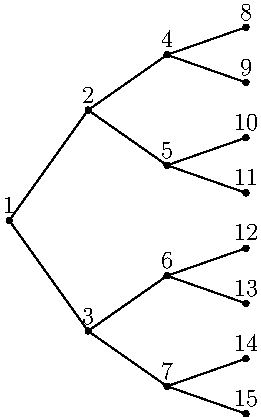
\includegraphics[width=0.29\textwidth]{bitree.pdf}
\parbox[b]{0.7\textwidth}{
\begin{itemize}
\item depth $\leftrightarrow$ time; position $\leftrightarrow$ spot price 
\item Node $\leftrightarrow$ path 
\item Visit nodes by Depth-first search alg.
\item $Pay_{\text{Node}} = (S_{\text{Node}}-K)^+$
\item $V_{\text{Node}} = Pay_{\text{Node}}$ for all leaves.
\item $E_{\text{Node}} =$ discounted value of weighted avg. of 
  the $Pay$ of children.
\item $V_{\text{Node}} = \max\Set{Pay_{\text{Nod}}, E_{\text{Node}}} $
\item The price at time $t=0$ is $V_{\text{root}}$
\end{itemize}
}
\end{frame}


%\subsection{Computational results for $\alpha$-quantile European option}
\begin{frame}{Numerical results for European quantile option}
\begin{table}
\caption{The price of European-style $\alpha$-quantile call options, with parameters
	$K=100, r=5\%, \sigma=0.2, \alpha=0.5, T=1$. }
\begin{center}
\begin{tabular}{l|lllllll}
 $S_0$ & $90$ & $95$ & $100$ & $105$ \\
\hline
28 steps & 1.60216 & 3.17876 & 5.61323 & 8.92661\\
30 steps & 1.60443 & 3.17806 & 5.61404 & 8.92702\\
32 steps & 1.60637 & 3.18346 & 5.61678 & 8.92718\\ 
34 steps & 1.60435 & 3.18426 & 5.61758 & 8.92875\\
36 steps & 1.60411 & 3.18846 & 5.61940 & 8.92925\\
\hline
Monte Carlo & 1.62450 & 3.21390 &  5.65385 & 8.96801 \\
Standard error & 0.00141 & 0.00200 & 0.00262 & 0.00317 \\
\hline
lookback & 9.45696 & 13.86499 & 19.16763 & 24.88215
\end{tabular}
\end{center}
\label{fig:euro5}
\end{table}%
\end{frame}

%\begin{frame}{Numerical results for European quantile option}
%\begin{table}
%\caption{The price of European-style $\alpha$-quantile call option,
%	with parameters
%	$K=95, r=5\%, \sigma=0.2, \alpha=0.8, T=0.25$. }
%\begin{center}
%\begin{tabular}{l|lllllll}
%$S_0$ & $95$ & $100$ & $105$        \\
%\hline
%26 steps & 4.59876 & 9.10824 & 14.1838 \\
%28 steps & 4.60931 & 9.11777 & 14.1954 \\
%30 steps & 4.61547 & 9.12485 & 14.2030 \\
%32 steps & 4.61816 & 9.12648 & 14.2054 \\
%34 steps & 4.61785 & 9.12676 & 14.2051 \\
%36 steps & 4.62050 & 9.12908 & 14.2079 \\
%\hline
%Monte Carlo & 4.66740 & 9.18266 & 14.26175\\
%Standard error & 0.00168 & 0.00200 &  0.00214\\
%\hline
%lookback & 8.381566 &  13.76059 & 19.13961
%\end{tabular}
%\end{center}
%\label{fig:euro8}
%\end{table}%
%\end{frame}


%\begin{frame}
%Under the Risk-Neutral framwork, the price of $\alpha$-quantile American call option
%is given by:
%\[
%V_t = \sup_{t \leq\tau\leq T}
%\mathbb{E}\left(e^{-r(T-\tau)}(S_0 e^{M(\alpha,T)} - K)^+|\mathcal{F}_t\right)
%\] 
%
%{\em Discuss:}
%\begin{itemize}
%\item Typical optimal stopping problem
%\item Discretized problem will give an approximation solution of the original. 
%\item The binomil tree method is doable, but no efficient.
%\end{itemize}
%\end{frame}

\subsection{An extrapolation improvement}

\begin{frame}{An extrapolation improvement}
\begin{itemize}
\item
Computational complexity: $2^{steps}$
\item
Problem: Hard to apply to large steps. 
\item
Solution: Richardson extrapolation
\begin{itemize}
\item
Basic idea: Suppose the tree method is of order $\vartheta$.  
\[
v(h) = v_0 + Ch^\vartheta + O(h^{\vartheta'}),
\]
where $v_0$ is the true value of the $\alpha$-quantile option and $\vartheta' > \vartheta$ .
\item
Two different step length $h_1, h_2$, $\eta = h_1/h_2$, 
\[
v_0= \frac{{\eta}^\vartheta v({h_1}/{\eta}) - v(h_1)}{{\eta}^\vartheta -1} + O(h_1^{\vartheta'}).
\]
\item
In our case: $\vartheta$,$h_1$, $h_2$?
\item
Using European price as standard to find the best set of {$\vartheta$,$h_1$, $h_2$}.
\end{itemize} 

\end{itemize}
\end{frame}

%\begin{frame}
%\begin{itemize}
%\item
%Basic idea: Suppose the tree method is of order $\vartheta$.  
%\[
%v(h) = v_0 + Ch^\vartheta + O(h^{\vartheta'}),
%\]
%where $v_0$ is the true value of the $\alpha$-quantile option and $\vartheta' > \vartheta$ .
%\item
%Two different step length $h_1, h_2$, $\eta = h_1/h_2$, 
%\[
%v_0= \frac{{\eta}^\vartheta v({h_1}/{\eta}) - v(h_1)}{{\eta}^\vartheta -1} + O(h_1^{\vartheta'}).
%\]
%\item
%In our case: $\vartheta$,$h1$, $h2$?
%\item
%Using European price as standard to find the best set of {$\vartheta$,$h1$, $h2$}.
%\end{itemize}
%\end{frame}
%






\begin{frame}{Computational results for $\alpha$-quantile American option}
\begin{table}[p]
\caption{The price of European-style $\alpha$-quantile call options, with parameters
	$S=100, K=100, r=5\%, \sigma=0.2, T=1$ and different $\alpha$. For extrapolation, $\vartheta=0.9$.}
\begin{center}
\begin{tabular}{l|lllll}
$\alpha$ & $0.5$ & $0.6$ & $0.7$ & $0.8$ & $0.9$       \\
\hline
18 steps  & 5.58991 & 7.02836 & 8.64998 & 10.5450 & 12.9325\\
36 steps  & 5.61940 & 7.07069 & 8.70835 & 10.6295 & 13.0804\\
\hline
Extrapolation  & 5.65345  & 7.11957  & 8.77575 & 10.72707 &13.25117 \\
\hline
Monte Carlo & 5.65519 &7.11064 & 8.77318 & 10.73129 & 13.24507\\
Standard eror &  0.00262 & 0.00303 & 0.00344 & 0.00386 & 0.00430    
\end{tabular}
\end{center}
\label{fig:euro9}
\end{table}%

\end{frame}

\begin{frame}{Computational results for $\alpha$-quantile American option}
\begin{table}[p]
\caption{The price of American-style $\alpha$-quantile call options, with parameters
	$S=100, K=100, r=5\%, \sigma=0.2, T=1$ and different $\alpha$. For extrapolation, $\vartheta=0.9$.  }
\begin{center}
\begin{tabular}{l|lllllll}
$\alpha$ & $0.5$ & $0.6$ & $0.7$ & $0.8$ & $0.9$       \\
\hline
%26 & 6.19546 & 7.65852 & 9.26385 & 11.1028 & 13.3703\\
%28 & 6.21365 & 7.67208 & 9.2838 & 11.1237 & 13.3911\\
%30 & 6.22887 & 7.68475 & 9.29502 & 11.1397 & 13.4019\\
%32 & 6.2432 & 7.69856 & 9.3113 & 11.1572 & 13.4248\\
%34 & 6.25529 & 7.71023 & 9.32278 & 11.168 & 13.4488\\
18 steps & 6.10629 & 7.57527 & 9.16086 & 10.9735 & 13.1843\\
36 steps & 6.26644 & 7.72127 & 9.32848 & 11.1789 & 13.4651\\
\hline
Extra & 6.45135 & 7.88984 & 9.52202 & 11.41606 & 13.78932 
\end{tabular}
\end{center}
\label{fig:amerc}
\end{table}%

\end{frame}




\section{Conclusion and further discussion}
\begin{frame}{Conclusion and further discussion}
\begin{itemize}
\item
Discretization error of Euler approximation
\begin{itemize}
\item Strong order from numerical study: for $\alpha=0$ or $\alpha=1$, $0.5$; for $0<\alpha<1$, around $0.75$.
\item Expected discretization error: $\alpha=0$ or $\alpha=1$, $O(1/N{1/2})$; $0<\alpha<1/2$ or $1/2<\alpha<1$ $O(1/N^{-1})$; $\alpha=1/2$, $0$; symmetry about $\mu=0$ and $\alpha=1/2$ and coefficient.
\item Future work: Theoretical study about the strong order of convergence.
\item Connect the price of discrete and continuous quantile options, probably by using the strong order of convergence. 
\end{itemize}
\item
Pricing of $\alpha$-quantile option
\begin{itemize} 
\item A tree method to price the European and American $\alpha$-quantile option at any time $t$. 
\item Future work: improve the efficiency. 
\end{itemize}
\end{itemize}
\end{frame}

\section{Reference}
\begin{frame}[allowframebreaks]{Reference}
\bibliography{prob}
\end{frame}

\end{document} 